%%%%%%%%%%%%%%%%%%%%%%%%%%%%%%%%%%%%%%%%%%%%%%%%%%%%%%%%%%%%%%%%%%%%%%%%%%%%%%%%%%%%
% Document data
%%%%%%%%%%%%%%%%%%%%%%%%%%%%%%%%%%%%%%%%%%%%%%%%%%%%%%%%%%%%%%%%%%%%%%%%%%%%%%%%%%%%
\documentclass[12pt]{article} %report allows for chapters
%%%%%%%%%%%%%%%%%%%%%%%%%%%%%%%%%%%%%%%%%%%%%%%%%%%%%%%%%%%%%%%%%%%%%%%%%%%%%%%%%%%%
\usepackage{preamble}

\begin{document}

\begin{center}
   \textsc{\large MATH 272, Homework 5, \emph{Solutions}}\\
   \textsc{Due March 9$^\textrm{th}$}
\end{center}
\vspace{.5cm}

\begin{problem}
A rough model of a molecular crystal can be described in the following way. Take the scalar function
\[
u(x,y)=\cos^2(x)+\cos^2(y).
\]
This function $u(x,y)$ describes the \emph{potential energy} for electrons in the crystal. Electrons are attracted to the areas with the smallest potential energy and move away from areas of high potential energy. 
\begin{enumerate}[(a)]
    \item Plot this function and include a printout.  Notice what this looks like.  You can imagine that each of the low points (well) is where a nucleus is located in the crystal.
    \item Plot the level curves where $u(x,y)=0$, $u(x,y)=\frac{1}{4}$, $u(x,y)=\frac{1}{2}$, and $u(x,y)=1$ for the range of values $-\frac{3\pi}{2}\leq x \leq \frac{3\pi}{2}$ and $-\frac{3\pi}{2}\leq y \leq \frac{3\pi}{2}$. 
    
    Picking the constant for the level curve tells you the \emph{kinetic energy} of the electron you are looking at.  It turns out that electrons (roughly) will orbit along these level curves.  Notice, some level curves bleed into the different troughs of neighboring molecules which means that electrons of sufficient energy happily flow through the crystal. However, electrons like to behave a bit differently thanks to their quantum nature!
    \item Find the gradient of this function $\grad u(x,y)$.
    \item At what point(s) is the gradient zero? \emph{Hint: Use your graph of the level curves to help.}
    \end{enumerate}
\end{problem}

\begin{solution}~
\begin{enumerate}[(a)]
    \item Here is the plot
    \begin{figure}[H]
        \centering
	\def\svgwidth{0.75\columnwidth}
	\input{Figures/crystal.pdf_tex}
    \end{figure}
    \item Here is the plot of the level curves.
    \begin{figure}[H]
        \centering
	\def\svgwidth{0.75\columnwidth}
	\input{Figures/level_curves.pdf_tex}
        \caption{Contour plot labeled with relevant values. Colors match the colors in the previous figure.}
    \end{figure}
    
    \item The gradient is
    \[
    \grad u(x,y) = \begin{pmatrix} -2\cos(x)\sin(x) \\ -2\cos(y)\sin(y) \end{pmatrix}.
    \]
    \item We want to find where
    \[
    \grad u(x,y) = \zerovec.
    \]
    This gives us two equations to work with:
    \begin{align}
        -2\cos(x)\sin(x) &= 0,\\
        -2\cos(y)\sin(y) &= 0.
    \end{align}
    Note that (1) is zero whenever $\cos(x)$ or $\sin(x)$ is zero, which happens at $x=\frac{n\pi}{2}$ for all integers $n$. Similarly, we have that (2) is zero when $y=\frac{m\pi}{2}$ for all integers $m$.  This gives us many different solutions in our given range of values.
    
    If we think graphically, these values where the gradient is zero occur at the tops and bottoms of the peaks and valleys respectively.  These are the maxima and minima of the function $u(x,y)$.
    
    However, not all of these solutions are solutions where the electrons will want to stay put.  We will have to work harder to find out which ones are minimizers of the energy!
\end{enumerate}
\end{solution}


\newpage
\begin{problem} 
Let us visualize vector fields using GeoGebra (specifically \url{https://www.geogebra.org/m/u3xregNW}). Plot the following vector fields and print them out. 
\begin{enumerate}[(a)]
    \item (Constant wind from the northwest) $\vecfieldV(x,y)=\begin{pmatrix} 1 \\ -1 \\ 0\end{pmatrix}$.
        \item (Two wind fronts meeting) $\vecfieldU(x,y,z)=\begin{pmatrix} y \\ x \\ 0 \end{pmatrix}$.
                        \item (Source) $\vecfieldE(x,y,z) = \begin{pmatrix} \frac{x}{(x^2+y^2+z^2)^{3/2}} \\ \frac{y}{(x^2+y^2+z^2)^{3/2}} \\ \frac{z}{(x^2+y^2+z^2)^{3/2}} \end{pmatrix}$.
                  \item (Vortex) $\boldsymbol{\vec{S}}(x,y,z)=\begin{pmatrix} \frac{-y}{x^2+y^2+z^2} \\ \frac{x}{x^2+y^2+z^2} \\ 0\end{pmatrix}.$           
\end{enumerate}
\end{problem}

\begin{solution}~
\begin{enumerate}[(a)]
    \item 
    \begin{figure}[H]
        \centering
        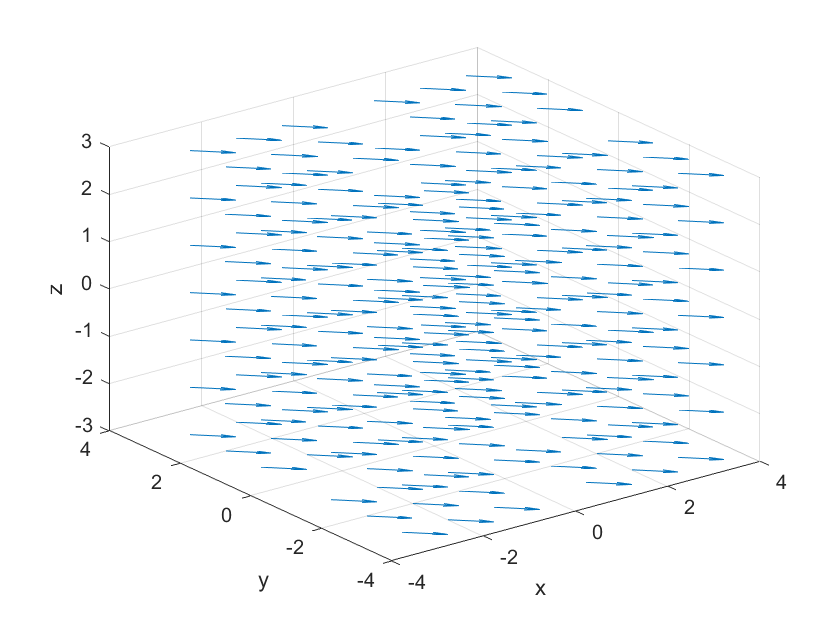
\includegraphics[width=.6\textwidth]{Figures/const_wind.png}
        \caption{Plot for $\vecfieldV(x,y,z)$.}
    \end{figure}
    \item 
    \begin{figure}[H]
        \centering
        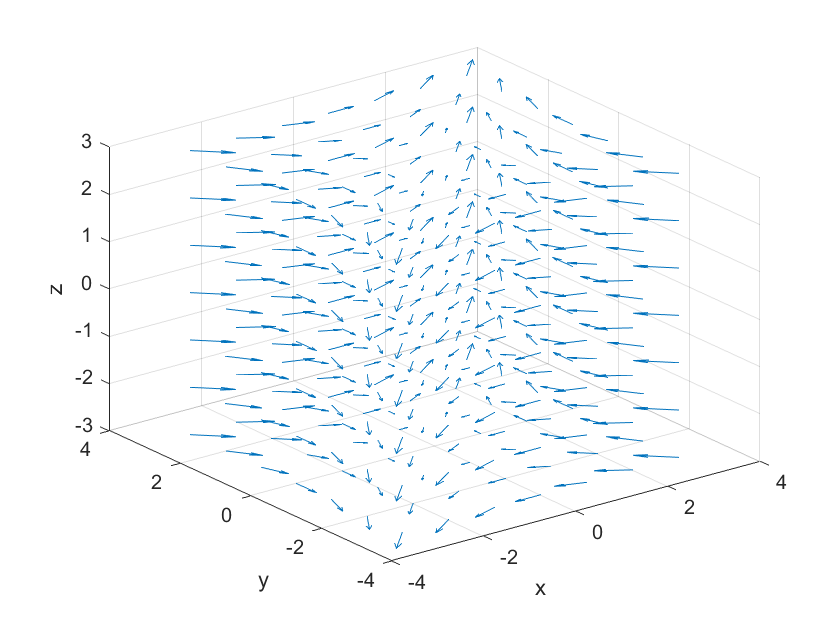
\includegraphics[width=.6\textwidth]{Figures/wind_fronts.png}
        \caption{Plot for $\vecfieldU(x,y,z)$.}
    \end{figure}
    \item 
    \begin{figure}[H]
        \centering
        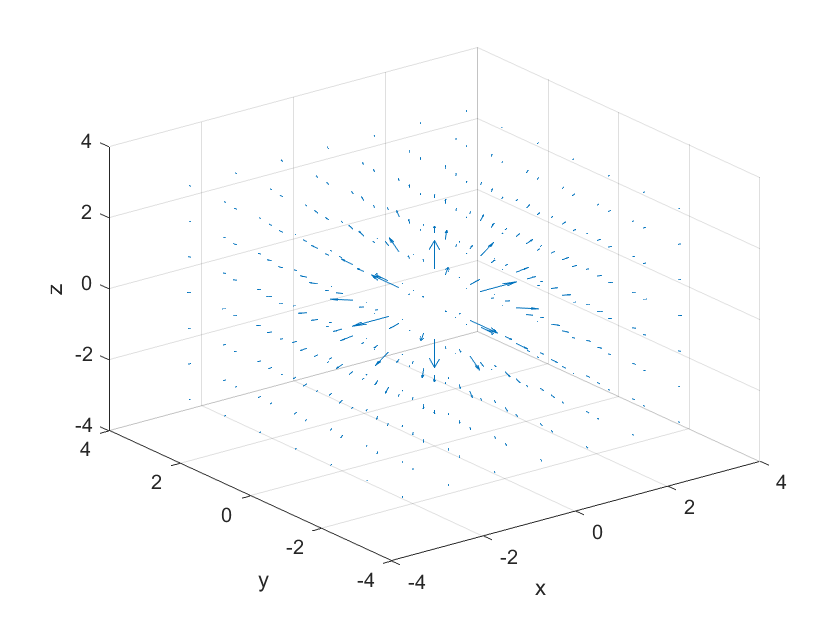
\includegraphics[width=.6\textwidth]{Figures/source.png}
        \caption{Plot for $\vecfieldE(x,y,z)$.}
    \end{figure}
    \item 
    \begin{figure}[H]
        \centering
        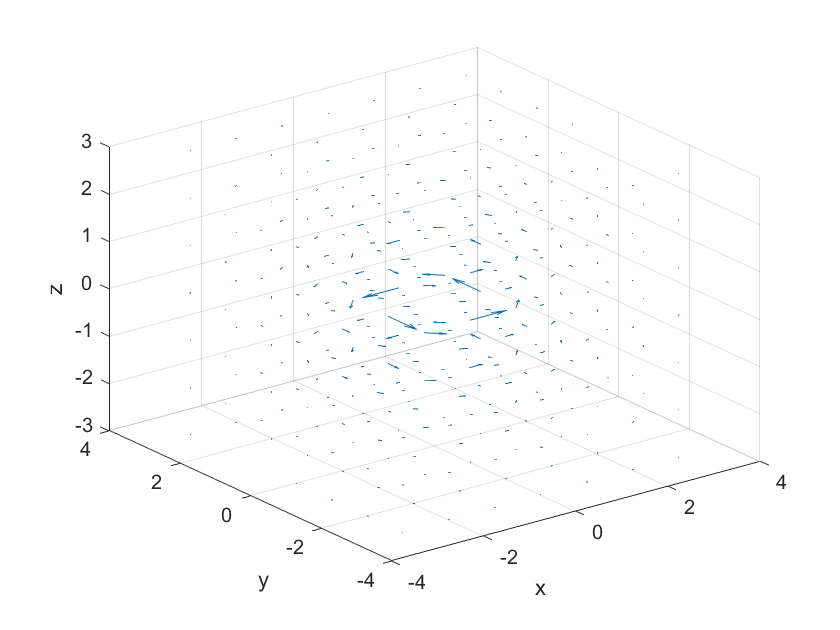
\includegraphics[width=.6\textwidth]{Figures/vortex.png}
        \caption{Plot for $\boldsymbol{\vec{S}}(x,y,z)$.}
    \end{figure}
\end{enumerate}
\end{solution}

\newpage
\begin{problem}
Compute the divergence and curl of the Source and Vortex fields from the previous problem.  What can we say about the divergence and curl of these fields at the origin?
\end{problem}
\begin{solution}
    First, let us take the curl of $\vecfieldE$.  We have
    \begin{align*}
        \grad \times \vecfieldE &= \begin{pmatrix} \frac{\partial E_3}{\partial y} - \frac{\partial E_2}{\partial z} \\ \frac{\partial E_1}{\partial z} -\frac{\partial E_3}{\partial 1} \\ \frac{\partial E_2}{\partial x} - \frac{\partial E_1}{\partial y} \end{pmatrix}\\
        &= \begin{pmatrix} \frac{-3yz}{(x^2+y^2+z^2)^{5/2}} - \frac{-3yz}{(x^2+y^2+z^2)^{5/2}} \\ \frac{-3xz}{(x^2+y^2+z^2)^{5/2}} - \frac{-3xz}{(x^2+y^2+z^2)^{5/2}} \\
        \frac{-3xy}{(x^2+y^2+z^2)^{5/2}} -\frac{-3xy}{(x^2+y^2+z^2)^{5/2}} \end{pmatrix}\\
        &= \begin{pmatrix} 0 \\ 0 \\ 0 \end{pmatrix}.
    \end{align*}
    At the origin, this curl is also identically zero.  The curl of $\vecfieldE$ is simply zero everywhere.
    
    Next, the curl of $\boldsymbol{\vec{S}}$,
        \begin{align*}
            \grad \times \boldsymbol{\vec{S}} &= \begin{pmatrix} 0 - \frac{-2xz}{(x^2+y^2+z^2)^2} \\ \frac{2yz}{(x^2+y^2+z^2)^2} - 0 \\
            \frac{-x^2+y^2+z^2}{(x^2+y^2+z^2)^2}- \frac{x^2-y^2+z^2}{(x^2+y^2+z^2)^2}\end{pmatrix}\\
            &= \begin{pmatrix}  \frac{2xz}{(x^2+y^2+z^2)^2} \\ \frac{2yz}{(x^2+y^2+z^2)^2} \\ \frac{z^2}{(x^2+y^2+z^2)^2}. \end{pmatrix}.
        \end{align*}
    Note that at the origin, we have a discontinuity.  Specifically, the curl at the origin will go to infinity (in each direction) at the origin since the numerator of each component of the curl is of lesser degree (2) than the denominator (4).
    
    The divergence of $\vecfieldE$ is
    \begin{align*}
        \grad \cdot \vecfieldE &= \frac{\partial E_1}{\partial x} + \frac{\partial E_2}{\partial y} + \frac{\partial E_3}{\partial z}\\
        &= \frac{-2x^2+y^2+z^2}{(x^2+y^2+z^2)^{5/2}} + \frac{x^2-2y^2+z^2}{(x^2+y^2+z^2)^{5/2}} + \frac{x^2+y^2-2z^2}{(x^2+y^2+z^2)^{5/2}}\\
        &= 0.
    \end{align*}
    It appears that the divergence of this field $\vecfieldE$ is zero, however we will see in Problem 5 that this isn't entirely true!
    
    Similarly, the divergence of $\boldsymbol{\vec{S}}$
    \begin{align*}
        \grad \cdot \boldsymbol{\vec{S}} &= \frac{2xy}{(x^2+y^2+z^2)^2} + \frac{-2xy}{(x^2+y^2+z^2)^2}\\
        &=0.
    \end{align*}
    Once again, this appears to be zero everywhere (including the origin). But one should be weary of whether or not this is totally true!
   
\end{solution}


\newpage
\begin{problem}
Consider the function
\[
f(x,y)=\sin\left(\frac{2\pi x}{5}\right)\sin\left(\frac{2\pi y}{5}\right).
\]
comes up when you want to find out how a square shaped drum head will vibrate when hit. 
\begin{enumerate}[(a)]
    \item Plot this function on the region $\Omega$ given by $0\leq x \leq 5$ and $0\leq y \leq 5$.  
    \item What is the value the function $f(x,y)$ on the boundary of the given region $\Omega$ (i.e, when $x=0$, $x=5$, $y=0$, and $y=5$)?
    \item Show that $f(x,y)$ is an eigenfunction of the Laplacian $\Delta = \grad \cdot \grad$. What is the eigenvalue?
\end{enumerate}
\end{problem}
\begin{solution}~
\begin{enumerate}[(a)]
    \item Here is the plot of the vibrating square drum head:
    \begin{figure}[H]
        \centering
	\def\svgwidth{0.75\columnwidth}
	\input{Figures/drum_head.pdf_tex}
    \end{figure}
    \item When $x=0$ we have
    \[
    f(0,y) = \sin\left( \frac{2\pi 0}{5}\right) \sin\left(\frac{2\pi y}{5}\right) = 0.
    \]
    Similarly, when $x=5$ $f(5,y)=0$, when $y=0$ $f(x,0)=0$, and when $y=5$ $f(x,5)=0$. 
    
    These are the boundary of the drum head.  That is, where the head of the drum is clamped down.
    
    \item We have
    \begin{align*}
        \frac{\partial f}{\partial x} &= \frac{2\pi}{5} \cos \left( \frac{2\pi x}{5} \right) \sin \left( \frac{2\pi y}{5} \right),\\
        \frac{\partial^2 f}{\partial x^2} &= \frac{-4\pi^2}{25} \sin \left( \frac{2\pi x}{5} \right) \sin \left( \frac{2\pi y}{5} \right),\\
        \frac{\partial f}{\partial y} &= \frac{2\pi}{5} \sin \left( \frac{2\pi x}{5} \right) \cos \left( \frac{2\pi y}{5} \right),\\
        \frac{\partial^2 f}{\partial y^2} &= \frac{-4\pi}{25} \sin \left( \frac{2\pi x}{5} \right) \sin \left( \frac{2\pi y}{5} \right).
    \end{align*}
    Then we have
    \[
    \frac{\partial^2 f}{\partial x^2} + \frac{\partial^2 f}{\partial y^2} = -\frac{8\pi^2}{25} \sin \left( \frac{2\pi x}{5} \right) \sin \left( \frac{2\pi y}{5} \right) = -\frac{8\pi^2}{25} f(x,y).
    \]
    So, the way a drum head vibrates is an eigen-problem.
\end{enumerate}
\end{solution}

\newpage
\begin{problem}
Consider the following vector field
\[
\vecfieldE(x,y,z) = \begin{pmatrix} \frac{x}{(x^2+y^2+z^2)^{3/2}} \\ \frac{y}{(x^2+y^2+z^2)^{3/2}} \\ \frac{z}{(x^2+y^2+z^2)^{3/2}} \end{pmatrix},
\]
which models the electric field of an proton (in units of of charge $q=1$) placed at the origin.
\begin{enumerate}[(a)]
	\item Show that $\vecfieldE(x,y,z) = - \grad V(x,y,z)$ where $V(x,y,z) = \frac{1}{\sqrt{x^2+y^2+z^2}}$.  We refer to $V(x,y,z)$ as the electrostatic potential or voltage.
	\item Let $\Omega$ be a box with side lengths two centered at the origin.  Compute the total flux of $\vecfieldE$ through the surface of the box $\Sigma$. That is,
	\[
	\int_\Gamma \vecfieldE(x,y,z) \cdot \unitvec d\Sigma.
	\]
 	\item Does the total flux depend on the size or shape of the box?
	\item Using the provided argument, one can compute
	\[
	\int_\Omega \grad \cdot \vecfieldE(x,y,z) d\Omega.
	\]
	\begin{itemize}
		\item Compute $\grad \cdot \vecfieldE$ and note that this is zero everywhere except at $(x,y,z)=(0,0,0)$.
		\item Note that the two integrals in this problem are equal. This is known as the \emph{divergence theorem} and it is a special case of a more general theorem called \emph{Stokes' theorem} which generalizes the fundamental theorem of calculus. Hence, you can now argue why
		\[
		\grad\cdot \vecfieldE = 4\pi\delta(x,y,z),
		\]
		where $\delta(x,y,z)$ is the 3-dimensional Dirac delta.
	\end{itemize}
\end{enumerate}
\end{problem}
\begin{solution}
    \begin{enumerate}[(a)]
        \item   We compute $-\grad V$,
        \begin{align*}
            -\grad V &= \begin{pmatrix} -\frac{\partial V}{\partial x} \\ -\frac{\partial V}{\partial y} \\ -\frac{\partial V}{\partial z} \end{pmatrix}\\
            &= \begin{pmatrix} \frac{x}{(x^2+y^2+z^2)^{3/2}} \\ \frac{y}{(x^2+y^2+z^2)^{3/2}} \\ \frac{z}{(x^2+y^2+z^2)^{3/2}} \end{pmatrix}.
        \end{align*}
        \item This portion requires computing six different (however, symmetric) integrals.  One can reduce the argument down to a single integral via a bit of physical/mathematical reasoning. Note that the field $\vecfieldE$ is radially symmetric in that the field points radially outward from the origin and the strength falls off as we move away from the origin.  Fundamentally, this means that each face of the cube receives the same amount of flux through it.
        
        Picture the situation as follows. We have the cube surface broken up into $6$ faces. We will label these faces as $\Sigma_1$, $\Sigma_2,\dots,\Sigma_6$.  
        \begin{figure}[H]
        	\centering
        	\def\svgwidth{0.75\columnwidth}
        	\input{Figures/cube_coordinate_axes.pdf_tex}
        \end{figure}
        One can take $\Sigma_4$, $\Sigma_5$, and $\Sigma_6$ to be the faces opposite to $\Sigma_1$, $\Sigma_2$ and $\Sigma_3$ respectively.  Each face then has a unique outward normal vector which we can denote by $\unitvec_{\Sigma_j}$ for the face $\Sigma_j$.
        \begin{figure}[H]
        	\centering
        	\def\svgwidth{0.75\columnwidth}
        	\input{Figures/cube_normal_vectors.pdf_tex}
        \end{figure}
        Thus, our integral over the cubic surface $\Sigma$ is given by
        \[
        \iint_{\Sigma} \vecfieldE \cdot \unitevec d\Sigma = \sum_{j=1}^6 \iint_{\Sigma_j} \vecfieldE \cdot \unitvec_{\Sigma_j}d\Sigma_j.
        \]
        By the symmetry argument before, we can simplify this further as
        \[
        \iint_\Sigma \vecfieldE \cdot \unitvec d\Sigma = 6 \iint_{\Sigma_1} \vecfieldE \cdot \unitvec_{\Sigma_1}d\Sigma_1.
        \]
        Now, we can evaluate this integral
        \begin{align*}
            6\iint_{\Sigma_1} \vecfieldE \cdot \unitvec_{\Sigma_1}d\Sigma_1 &= \int_{-1}^1 \int_{-1}^1 \vecfieldE(x,y,1) \cdot \zhat dxdy\\&= 6\int_{-1}^1 \int_{-1}^1 \frac{1}{(x^2+y^2+1)^{3/2}}dxdy\\
                &= 6\int_{-1}^1 \frac{2}{(y^2+1)\sqrt{y^2+2}} dy\\
                &= 6\frac{2\pi }{3}\\
                &= 4\pi.
        \end{align*}
    \end{enumerate}
    \item Note that the divergence of $\vecfieldE$ is zero everywhere aside from the origin.  Hence, the only possible source of flux comes from the origin and our previous argument discussed the symmetry of this field.  So long as we integrate in a surface that encloses the origin, we will have the same answer.  This leads us to (d).
    \item We have already computed $\grad \cdot \vecfieldE$ and noted this in an earlier problem.  It's now very physically reasonable to suspect that we have the following identity
    \[
    \int_\Omega \grad \cdot \vecfieldE d\Omega = \int_\Sigma \vecfieldE \cdot \unitvec d\Sigma,
    \]
    since the amount of ``source behavior" in the region $\Omega$ should directly correspond to the flux that will pass through the boundary.  To picture this literally, if we pump in water at $(0,0,0)$, we know how much water we pumped in by seeing how much flows through any surface surrounding the origin.  
    
    Thus, our argument is that
    \[
    \int_\Omega \grad \cdot \vecfieldE d\Omega = 4\pi.
    \]
    Now, $\grad\cdot \vecfieldE$ is zero aside from at $(x,y,z)=(0,0,0)$, and thus $\grad \cdot \vecfieldE$ must mimic the Dirac delta by being infinite at the origin (which we observed previously).  Hence, we conclude that
    \[
    \grad \cdot \vecfieldE = 4\pi \delta(x,y,z).
    \]
    Furthermore, if we relate this to the Maxwell equation for the electric field $\vecfieldE$ due to a charge distribution $\rho(x,y,z)$, i.e.,
    \[
    \grad \cdot \vecfieldE = \rho/\epsilon_0,
    \]
    we see that a point charge corresponds to a distribution $\delta(x,y,z)$ times some constant.
\end{solution}

\end{document}